% Manual for Tali Forth for the 65c02
% Scot W. Stevenson <scot.stevenson@gmail.com>
% First version: 02. Mar 2018
% This version: 20. May 2018
% See:
% - https://en.wikibooks.org/wiki/LaTeX/Document_Structure#Document_classes
% - https://www.sharelatex.com/blog/2013/08/02/thesis-series-pt1.html
% Install additional fonds with "sudo apt-get install texlive-fonts-extra"
% https://launchpad.net/ubuntu/xenial/+package/texlive-fonts-extra
\documentclass[a4paper,notitlepage]{report}
\usepackage[width=150mm,top=25mm,bottom=25mm]{geometry}
\usepackage{fancyhdr}
\pagestyle{fancy}

\usepackage{graphicx}
\usepackage{makeidx}
\makeindex

\usepackage{sourcecodepro}      % for monospaced

\usepackage{listings}
\lstset{basicstyle=\ttfamily,breaklines=true} % use monospace

\usepackage{color}
\usepackage[colorlinks=true]{hyperref}   % must be last

% Add real titlepage

\title{The Tali Forth 2 Manual (ALPHA)}
\author{Scot W.~Stevenson}
\date{\today}


% --------------------------------
\begin{document}

\maketitle

\begin{abstract}
        Tali Forth 2 is a bare-metal ANSI(ish) Forth for the 65c02 8-bit MPU. 
        It aims to be, roughly in order of importance: 

        \begin{description}

        \item [Easy to try.]
                \href{https://github.com/scotws/TaliForth2}{Download the source}
                -- or even just the binary -- and you can immediately
                run it in an emulater. This lets you experiment with a
                working 8-bit Forth for the 65c02 without any special
                configuration.

        \item [Simple.] The subroutine-threaded (STC) design and happily
                overcommented source code give hobbyists the chance to study a
                working Forth at the lowest level. The manual -- this
                document -- explains structure and code in detail. The aim
                is to make it easy to port Tali Forth 2
                to various 65c02 hardware projects.

        \item [Specific.] Many Forths available are `general' implementations with
                a small core adapted to the target processor. Tali Forth 2 was
                written as a "bare metal Forth" for the 65c02 8-bit MPU
                and that MPU only, with its strengths and limitations in
                mind.

        \item [Standardized.] Most Forths available for the 65c02 are based on ancient,
                outdated templates such as FIG Forth. Learning Forth with them is like
                trying to learn modern English by reading Chaucer. Tali
                Forth (mostly) follows the current ANSI Standard.
\end{description}

        Tali Forth is hosted at GitHub at
        \href{https://github.com/scotws/TaliForth2}{https://github.com/scotws/TaliForth2}. 
        The discussion thread is at 6502.org at
        \href{http://forum.6502.org/viewtopic.php?f=9\&t=2926}{http://forum.6502.org/viewtopic.php?f=9\&t=2926}.
        
\end{abstract}

% --------------------------------
\tableofcontents
\listoffigures
\listoftables

% --------------------------------
\part{Introduction}

\chapter{Why}
        % The Why of Tali Forth
% Scot W. Stevenson

\begin{quote}
        Forth is well suited to resource-constrained situations. It doesn't need
        lots of memory and doesn't have much overhead. It can take full
        advantage of whatever hardware or interfaces exist.
\end{quote}
\begin{flushright}
        -- Charles Moore,\index{Moore, Charles} 
        \href{https://www.red-gate.com/simple-talk/opinion/geek-of-the-week/chuck-moore-geek-of-the-week/}{`Chuck
        Moore: Geek of the Week', redgate Hub 2009}
\end{flushright}

\section{The big picture}

This section provides background information on Forth, the 6502 processor, and
why anybody would want to combine the two. It can be safely skipped if you
already know all those things.

\subsection{The 6502 MPU}

It is a well-established fact that humanity reached the apex of processor design
with the 6502\index{6502} in 1976. Created by a team including Chuck
Peddle\index{Peddle, Chuck} and Bill Mensch\index{Mensch, Bill}, it was the
engine that powered the 8-bit home computer revolution of the
1980s.\footnote{Rumor has it that there was another MPU called `Z80'\index{Z80},
but it ended up being a mere footnote.} The VIC-20\index{VIC-20}, Commodore
PET\index{Commodore PET}, Apple II\index{Apple II}, and Atari 800\index{Atari
800} all used the 6502, among others. 

\begin{figure}[h !]
        \centering
        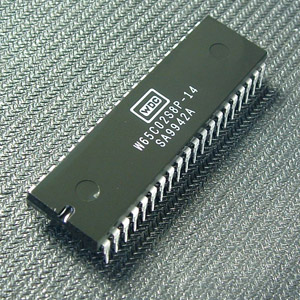
\includegraphics[width=0.5\textwidth]{pics/W65c02}
        \caption{\textit{The 65c02 MPU.} Photo: Anthony King, released in 
        the public domain}
        \label{fig:65c02}
\end{figure}

More than 40 years later, the processor is still in production by the \href
{http://www.westerndesigncenter.com/wdc/w65c02s-chip.cfm}{Western Design
Center}\index{WDC}. Apart from commercial uses, there is an active hobbyist
scene centered on the website \href{http://6502.org/}{6502.org}.\index{6502.org}
Quite a number of people have built their own 8-bit computers based on this chip
and the instructions there, including a
\href{http://wilsonminesco.com/6502primer/}{a primer} by Garth
Wilson\index{Wilson, Garth}. It is for these systems that Tali Forth 2 was
created.

The most important variant of the 65c02 produced today is the \href
{https://en.wikipedia.org/wiki/WDC\_65C02}{65c02}\index{65c02}, a CMOS chip with
some additional instructions. It is for this chip that Tali Forth 2 was written. 

But why program in 8-bit assembler at all?\footnote{Wilson\index{Wilson,
Garth} answers this question in greater detail as part of his
\href{http://wilsonminesco.com/6502primer/65tutor\_intro.html}{6502 primer}} The
65c02 is fun to work with because of its clean instruction set architecture
(ISA)\index{instruction set!architecture}\index{ISA|see {instruction set}}. This
is not the place to explain the joys of assembler. The official handbook for the
65c02 is \textit{Programming the 65816, including the 6502, 65C02 and
65802}\cite{eyeslichty}.


\subsection{Forth}

\begin{quote}
        If C gives you enough rope to hang yourself, Forth is a flamethrower
        crawling with cobras.
\end{quote}
\begin{flushright}
        -- Elliot Williams,\index{Williams, Elliot} \href{https://hackaday.com/2017/01/27/forth-the-hackers-language/}{
        \textit{Forth: The Hacker's Language}}
\end{flushright}

Forth\index{Forth|textbf} is the \textit{enfant terrible} of programming
languages. It was invented by Charles `Chuck' Moore\index{Moore, Charles} in the
1960s to do work with radio astronomy, way before there were modern operating
systems or programming languages.\footnote{A brief history of Forth can be found
at \href{https://www.forth.com/resources/forth-programming-language/}
{https://www.forth.com/resources/forth-programming-language/}} As a language for
people who actually need to get things done, it lets you run with scissors, play
with fire, and cut corners until you've turned a square into a circle. Forth is
not for the faint-hearted: It is trivial, for instance, to redefine 1 as 2 and
\texttt{true}\index{true@\texttt{true}} as
\texttt{false}.\index{false@\texttt{false}} Though you can do really, really
clever things with few lines of code, the result can be hard for other people to
understand, leading to the reputation of Forth begin a `write-only language'.
However, Forth excels when you positively, absolutely have to get something done
with hardware that is really too weak for the job. 

It should be no surprise that NASA\index{NASA} is one of the organizations who
use Forth. The \textit{Cassini} mission\index{Cassini@\textit{Cassini}} to
Saturn used a
\href{http://www.cpushack.com/2013/02/21/charles-moore-forth-stack-processors/}{Forth
CPU}, for instance. It is also perfect for small computers like the 8-bit 65c02.
After a small boom in the 1980s, more powerful computers led to a decline of the
language. The `Internet of Things' with embedded small processors has led to a
certain amount
\href{https://www.embedded.com/design/programming-languages-and-tools/4431133/Go-Forth-}{renewed
interest} in the language. It helps that Forth is easy to implement: It is
stack-based, uses reverse polish notation (RPN)\index{RPN|see {reverse polish
notation}}\index{reverse polish notation} and a simple threaded\index{threading}
interpreter model. 

There is no way this document can provide an adiquate introduction to Forth.
There are quite a number of tutorials, however, such as \textit{A Beginner's
Guide to Forth} by J.V.~Nobel\cite{nobel} or the classic (but slightly dated)
\textit{Starting Forth}\cite{brodie03} by Leo Brodie\index{Brodie, Leo}.
Gforth,\index{Gforth} one of the more powerful free Forths, comes with its own
\href{http://www.complang.tuwien.ac.at/forth/gforth/Docs-html/Tutorial.html}{tutorial}.\footnote{Once
you have understood the basics of the language, do yourself a favor and read
\textit{Thinking Forth} by Brodie\cite{brodie84}\index{Brodie, Leo}, which deals
with the philosophy of the language. Like Lisp\index{Lisp}, exposure to Forth
will change the way you think about programming.} 


\section{Writing your own Forth}

Even if the 65c02 is great and Forth is brilliant, why got to the effort of
writing a new, bare-metal version of the languages? After almost 50 years,
shouldn't there be a bunch of Forths around already?


\subsection{FIG Forth}

In fact, the classic Forth availble for the whole group of 8-bit MPUs is FIG
Forth\index{FIG Forth} -- `FIG' stands for `Forth Interest Group'. Ported to
various architectures, it was original based on an incarnation for the 6502
written by Bill Ragsdale\index{Ragsdale, Bill} and Robert Selzer\index{Selzer,
Robert}. There are PDFs of the
\href{http://www.forth.org/fig-forth/fig-forth\_6502.pdf}{6502 version} from
September 1980 freely available -- Forths are traditionally placed in the public
domain -- and more than one hobbyist has revised it to his machine. 

However, Forth has changed a lot in the past three decades. There is now a
standardized version called \href{https://forth-standard.org/}{ANSI Forth
standard}\index{ANSI Forth}, which includes such basic changes as how the
\texttt{do} loop works. Learning the language with FIG Forth is like learning
English with \textit{The Canterbury Tales}.\index{Canterbury Tales,
The@\textit{Canterbury Tales, The}}


\subsection{A modern Forth for the 65c02}

Tali Forth was created to provide an easy to understand modern Forth written
especially for the 65c02 that anybody can understand, adapt to their own use,
and maybe actually work with. As part of that effort, the source code is heavily
commented. And this document tries to explain the internals in more detail.

% end


\chapter{Overview of Tali Forth}
        % Overview of Tali Forth
% Scot W. Stevenson

% -------------------------------------
\section{Design considerations}

When creating a new Forth, there are a bunch of design decisions to be
made.\footnote{The best introduction to these questions is found in
\href{http://www.bradrodriguez.com/papers/moving1.htm}{\textit{Design Decisions
in the Forth Kernel}} by Brad Rodriguez\index{Rodriguez, Brad}} Spoiler alert:
Tali Forth ended up as a subroutine-threaded variant with a 16-bit cell size and
a dictionary that keeps headers and code separate. If you don't care and just
want to use the program, skip ahead. 

\subsection{Characteristics of the 65c02}

Since this is a bare-metal Forth, the most important consideration is the target
processor. The 65c02 only has one full register, the accumulator
A\index{accumulator}, and two secondary registers X\index{X register} and
Y\index{Y register}. All are 8-bit wide. There are 256 bytes that are more
easily addressable on the Zero Page\index{Zero Page}. A single hardware stack is
used for subroutine jumps. The address bus\index{address bus} is 16 bits wide
for a maximum of 64 KiB of RAM\index{RAM} and ROM\index{ROM}. For the default,
simple setup, we assume 32 KiB of each. 

\subsection{Cell size}

The 16 bit address bus\index{address bus} suggests the cell size should be 16
bits as well. This is still easy enough to realize on a 8-bit MPU, though not as
comfortable as working with the 65816\index{65816}, the 65c02's big brother,
with an actual 16 bit register size.

\subsection{Threading technique}\index{threading}

A `thread' in Forth is simply a list of addresses of words to be executed. 
There are four basic threading techniques:\footnote{For the 8086 MPU, Guy
Kelly\index{Kelly, Guy} compared various Forth implementations in
1992\cite{kelly92}}

\begin{description}
        \item [Indirect threaded (ITC)] The oldest, original variant, used by FIG
                Forth\index{FIG Forth}. All other versions are modifications of this 
                model.
        \item [Direct threaded (DTC)] Includes more assembler code to speed
                things up, but slightly larger than ITC. 
        \item [Token threaded (TTC)] The reverse of DTC in that it is slower, but uses
                less space than the other Forths. Words are created as a table
                of tokens.
        \item [Subroutine threaded (STC)] This technique converts the words to a simple
                series of \texttt{jsr} combinations. 
\end{description}

Our lack of registers and the goal of creating a simple and easy to understand
Forth makes subroutine threading the most attractive solution. We will try to
mitigate the pain caused by the 12 cycle cost of each and every \texttt{jsr/rts}
combination by including a relatively large number of native words\index{native
words}. 

\subsection{Register use}

The lack of registers -- and 16 bit registers at that -- becomes apparent when
you realize that Forth classically uses at least four `virtual' registers:

\begin{table}[h !]
        \centering
        \label{tab:registers}
        \begin{tabular}{| c | l |}
                \hline
                W   & Working register\\
                IP  & Interpreter Pointer\\
                DSP & Data Stack Pointer\\
                RSP & Return Stack Pointer\\
                \hline
        \end{tabular}
        \caption{The classic Forth registers}
\end{table}

On a modern processor like a RISC-V\index{RISC-V} RV32I CPU with 32 registers of
32 bit each, this wouldn't be a problem. In fact, we'd be trying to figure out
what else we could keep in a register. On the 65c02, at least we get the RSP for
free with the built-in stack pointer. This still leaves three registers. We cut
that number down by one through subroutine threading, which gets rid of the IP.
For the DSP, we use the 65c02's Zero Page\index{Zero Page} indirect addressing
mode with the X register\index{X register}. This leaves W, which we put on the
Zero Page as well. 


\subsection{Data Stack design}

We'll go into greater detail on how the Data Stack works in a later chapter when
we look at the internals. Briefly, the stack is realized on the Zero
Page\index{Zero Page} for speed. For stability, we provid underflow
checks\index{underflow!detection} in the relevant words, but give the user the
option of stripping it out for native compilation\index{native compilation}.


\subsection{Dictionary structure}

Each Forth word consists of the actual code and the header\index{header} which
holds the meta-data. Part of this data is the single-linked list of words which
is searched. 

In constrast to Tali Forth 1\index{Tali Forth 1}, which kept the header and body
of the words together, Tali Forth 2 keeps them separate. This lets us play
various tricks with the code to make it more effective.

\subsection{Deeper down the rabbit hole}

This concludes our overview of the basic Tali Forth 2 structure. For those
interested, a later chapter will provide far more detail.


% --------------------------------
\part{User Guide}

\chapter{Installing}
        % Installing Tali Forth 2
% This version: 03. May 2018
\section{Downloading}

Tali Forth was created to be easy to get started with. In fact, all you should
need is the \texttt{ophis.bin} binary file and the
\texttt{py65mon}\index{py65mon@\texttt{py65mon}} simulator.

\subsection{Downloading Tali Forth}

The newest version of Tali Forth 2 lives on GitHub\index{GitHub} at
\href{https://github.com/scotws/TaliForth2}{https://github.com/scotws/TaliForth2}.
You can either clone the code with \texttt{git}\index{git@\texttt{git}} or
simply download it. To just try the program, all you need is the
\texttt{taliforth-py65mon.bin} binary. 

\subsection{Downloading the py65mon Simulator}\index{py65mon|textbf}

Tali was written to run out of the box on the 
\texttt{py65mon} simulator from
\href{https://github.com/mnaberez/py65}{https://github.com/mnaberez/py65}. This
is a Python\index{Python} program that should run on various operating systems. 

To install py65mon on Linux\index{Linux}, use the command \texttt{sudo pip
install -U py65}. If you don't have PIP\index{PIP} installed, you will have to
add it first with \texttt{sudo apt-get install python-pip}.  There is a
\texttt{setup.py} script as part of the package.

\section{Running the binary}

To start the emulator, run:
\begin{lstlisting}[frame=lines]
        py65mon -m 65c02 -r taliforth-py65mon.bin
\end{lstlisting}

\noindent Note that the option \texttt{-m 65c02} is required, because Tali Forth
makes extensive use of the additional commands of the CMOS version and will not
run on a stock 6502 MPU.



\chapter{Running}
        % Chapter Running Tali Forth 2
% Scot W. Stevenson
% This version 01. June 2018

\begin{quote}
	One doesn't write programs in Forth. Forth is the program.
\end{quote}
\begin{flushright}
        -- Charles Moore,\index{Moore, Charles} \textit{Masterminds of Programming}\cite{biancuzzi09}
\end{flushright}


% -------------------------------------------------
\section{Booting}\index{booting}

Out of the box, Tali Forth boots a minimal kernel\texttt{kernel}\index{kernel}
to connect to the py65mon\index{py65mon} simulator. By default, this stage ends
with a line such as

\begin{lstlisting}[frame=lines]
        Tali Forth 2 default kernel for py65mon (18. Feb 2018)
\end{lstlisting}

When you port Tali Forth to your own hardware, you'll have to include your own
kernel (and probably should print out a different line).

\noindent Tali Forth itself boots next, and after setting up various internal
things, compiles the high level words. This causes a slight delay, depending on
the number and length of these words. As the last step, Forth should spit out a
boot string like

\begin{lstlisting}[frame=lines]
        Tali Forth 2 for the 65c02
        Version ALPHA 07. Mar 2018 
        Copyright 2014-2018 Scot W. Stevenson
        Tali Forth 2 comes with absolutely NO WARRANTY
        Type 'bye' to exit
\end{lstlisting}

\noindent Because these are the last high-level commands Tali Forth executes,
this functions as a primitive self-test. If you have modified the high level
Forth words\index{Forth words} in either \texttt{forth\_words.fs} or
\texttt{user\_words.fs}, the boot process might fail with a variant of the error
message `unknown word'. The built-in, native words should always work. For this
reason, \texttt{dump}\index{dump@\texttt{dump}} is a built-in word -- it very
useful for testing.


% -------------------------------------------------
\section{Available words}

Tali Forth comes with the following Forth words\index{Forth words} out of the
box:

\begin{lstlisting}[frame=lines]
        see within to d.r d. ud.r ud. .r u.r */mod */ mod /mod /
        action-of is defer@ defer! while until repeat else then
        if .( ( drop dup swap ! @ over >r r> r@ nip rot -rot tuck
        , c@ c! +! execute emit type . u. ? false true space 0 1
        2 2dup ?dup + - abs dabs and or xor rshift lshift pick char
        [char] char+ chars cells cell+ here 1- 1+ 2* = <> < > 0=
        0<> 0> 0< min max 2drop 2swap 2over 2variable 2r@ 2r> 2>r
        invert negate dnegate c, bounds spaces bl -trailing /string
        refill accept unused depth key allot create does> variable
        constant value s>d d>s d- d+ erase blank fill find-name '
        ['] name>int int>name name>string >body defer latestxt
        latestnt parse-name parse source source-id : ; compile, [ ]
        0branch branch literal sliteral ." s" postpone immediate
        compile-only never-native always-native nc-limit abort
        abort" do ?do i j loop +loop exit unloop leave recurse quit
        begin again state evaluate base digit? number >number hex
        decimal count m* um* * um/mod ud/mod sm/rem fm/mod \ move
        cmove> cmove pad >in <# # #s #> hold sign output input cr
        page at-xy marker words wordsize aligned align bell dump .s
        find word cold bye
\end{lstlisting}

\noindent (Call \texttt{words}\index{words@\texttt{words}} in Tali Forth for the
current list.)

Though the list might look unsorted, it actually reflects the priority in the
dictionary\index{dictionary}, that is, which words are found first. For
instance, the native words\index{native words} -- those coded in assembler --
start with \texttt{drop}\index{drop@\texttt{drop}}
\texttt{bye}\index{bye@\texttt{bye}}, which is the last word that Tali Forth
will find.\footnote{If you're going to quit, speed can't be that important} The
words before \texttt{drop} are those that are defined in high-level Forth. For
more information on the words, use the \texttt{see}\index{see@\texttt{see}}
command.

Note that the built-in words are lower case\index{case!lower}. Newly defined
words can be in any case and will be distinct -- `KASUMI' is a different word
than `Kasumi'.\index{Goto, Kasumi}


\subsection{History}\index{history, command line}

Tali's command line includes a simple, eight-element history function. To
access the previous entries, press \texttt{CONTROL-p}, to go forward to the next
entry, press \texttt{CONTROL-n}. 


\subsection{Standards}

Tali Forth is orientated on ANSI Forth, but (currently) doesn't contain the
complete set of even the core words. Tali also adopted some words from
Gforth\index{Gforth} such as \texttt{bounds}\index{bounds@\texttt{bounds}}. In
practical terms, Tali aims to be a subset of Gforth: If a program runs on Tali,
it should run on Gforth the same way or have a very good reason not to. 

In addition, there are a few words that are specific to Gforth such as 
\texttt{nc-limit}\index{nc-limit@\texttt{nc-limit}}. 


\subsection{Tali Forth special words}

Tali Forth includes a number of words not found in Gforth or ANSI Forth. 

\begin{itemize}

        \item \textbf{\texttt{0branch}}\index{0branch@\texttt{0branch}} \texttt{( f -- )} 
                Take branch if TOS is zero. Used internally for branching
                commands such as \texttt{if}\index{if@\texttt{if}}. This is
                usually replaced by
                \texttt{cs-pick}\index{cs-pick@\texttt{cs-pick}} and 
                \texttt{cs-roll}\index{cs-roll@\texttt{cs-roll}} in modern
                Forths; Tali Forth might switch to this model in the future.

        \item \textbf{\texttt{0}}\index{0@\texttt{0}} \texttt{( -- 0 )} 
                Push the number 0 on the Data Stack.

        \item \textbf{\texttt{1}}\index{1@\texttt{1}} \texttt{( -- 1 )} 
                Push the number 1 on the Data Stack.

        \item \textbf{\texttt{2}}\index{2@\texttt{2}} \texttt{( -- 2 )} 
                Push the number 2 on the Data Stack.

        \item \textbf{\texttt{always-native}}\index{always-native@\texttt{always-native}}\texttt{( -- )} 
                Mark latest word so that it is always natively compiled. 
   
        \item \textbf{\texttt{bell}}\index{bell@\texttt{bell}} \texttt{( -- )} 
                Ring the terminal bell (print ASCII\index{ASCII} 07)

        \item \textbf{\texttt{branch}}\index{branch@\texttt{branch}}\texttt{( -- )} 
                Always take branch. Used internally for branching commands such
                as \texttt{if}\index{if@\texttt{if}}. This is usually replaced
                by \texttt{cs-pick}\index{cs-pick@\texttt{cs-pick}} and
                \texttt{cs-roll}\index{cs-roll@\texttt{cs-roll}} in modern
                Forths; Tali Forth might switch to this model in the future.

        \item \textbf{\texttt{compile-only}}\index{compile-only@\texttt{compile-only}}
                \texttt{( -- )} Mark latest word as compile only.

        \item \textbf{\texttt{digit?}}\index{digit?@\texttt{digit?}} 
                \texttt{( char -- u f | char f )} If character is a digit,
                convert and set a success flag, otherwise return the character
                and a failure flag.

        \item \textbf{\texttt{input}}\index{input@\texttt{input}} \texttt{( -- addr )} 
                Return the address where the vector for the input routine is
                stored (not the vector itself). Used for input redirection for 
                \texttt{emit}\index{emit@\texttt{emit}} and others. 

        \item \textbf{\texttt{int>name}}\index{int>name@\texttt{int>name}} \texttt{( xt -- nt )} 
                Given the execution token\index{execution token} of a
                word, return the name token.\index{name token}. 
                
        \item \textbf{\texttt{latestnt}}\index{latestnt@\texttt{latestnt}} \texttt{( -- nt )} 
                Return the last used name token\index{name token}. The Gforth
                version of this word is called
                \texttt{latest}\index{latest@\texttt{latest}}.

        \item \textbf{\texttt{nc-limit}}\index{nc-limit@\texttt{nc-limit}}\texttt{( -- addr )} 
                Return the address where the threshold value for native
                compiling\index{native compiling} is kept. To check the value of
                this parameter, use \texttt{nc-limit ?}. The default is 20.

        \item \textbf{\texttt{never-native}}\index{never-native@\texttt{never-native}} \texttt{( -- )} 
                Mark most recent word so it is never natively compiled.

        \item \textbf{\texttt{number}}\index{number@\texttt{number}} 
                \texttt{( addr u -- u | d )} Convert a string to a number.
                Gforth uses
                \texttt{s>number?}\index{s>number?@\texttt{s>number?}} instead
                and returns a success flag as well. 

        \item \textbf{\texttt{output}}\index{output@\texttt{output}} \texttt{( -- addr )} 
                Return the address where the vector for the output routine is
                stored (not the vector itself). Used for output redirection for 
                \texttt{emit}\index{emit@\texttt{emit}} and others. 

        \item \textbf{\texttt{uf-strip}}\index{uf-strip@\texttt{uf-strip}} \texttt{( -- addr )} 
                Return the address where the flag is kept that decides if
                the underflow\index{underflow} checks are removed during native
                compiling. To check the value of this flag, use 
                \texttt{uf-strip ?}.

        \item \textbf{\texttt{wordsize}}\index{wordsize@\texttt{wordsize}}
                \texttt{( nt -- u )} Given the name token \index{name token} of
                a Forth word, return its size in bytes. Used to help tune 
                native compiling\index{native compiling}.

\end{itemize}


% -------------------------------------------------
\section{Native compiling}\index{compiling!native}

As the name says, subroutine threaded code\index{threading} encodes the words as
a series of subroutine jumps. Because of the overhead caused by these jumps,
this can make the code slow. Therefore, Tali Forth enables `native compiling',
where the machine code from the word itself is included instead of a subroutine
jump. 

The parameter \texttt{nc-limit}\index{nc-limit@\texttt{nc-limit}} sets the limit
of how small words have to be to be natively compiled. To get the current value
(usually 20), check the value of the system variable: 

\begin{lstlisting}[frame=lines]
        nc-limit ?
\end{lstlisting}

\noindent To set a new limit, save the maximal allowed number of bytes in the
machine code like any other Forth variable:

\begin{lstlisting}[frame=lines]
        40 nc-limit !
\end{lstlisting}

To complete turn off native compiling, set this value to zero.


% -------------------------------------------------
\section{Underflow detection}\index{underflow!detection}

When a word tries to access more words on the stack than it is holding, an
`underflow' error occurs. Whereas Tali Forth 1\index{Tali Forth 1} didn't check
for these errors, this version does. 

However, this slows the program down. Because of this, the user can turn off
underflow detection for words that are natively compiled into new words. To do
this, set the system variable
\texttt{uf-strip}\index{uf-strip@\texttt{uf-strip}} to
\texttt{true}\index{true@\texttt{true}}. Note this does not turn off underflow
detection in the built-in words. Also, words with underflow detection which are
not included in new words through native compiling will also retain their tests.


% -------------------------------------
\section{Restarting}

Tali Forth has a non-standard word \texttt{cold}\index{cold@\texttt{cold}} that
resets the system. Note that this doesn't erase any data in memory, but just
moves the pointers back. When in doubt, you might be better off quitting and
restarting completely.


% -------------------------------------
\section{Gotchas}

Tali has a 16-bit cell size (use \texttt{1 cells 8 * .} to get the cells size in
bits with any Forth), which can trip up calculations when compared to the
\textit{de facto} standard Gforth\index{Gforth} with 64 bits. Take this example:

\begin{lstlisting}[frame=lines]
( Gforth )      decimal 1000 100 um* hex swap u. u.  186a0 0  ok
( Tali Forth)   decimal 1000 100 um* hex swap u. u.  86a0 1  ok
\end{lstlisting}

\noindent Tali has to use the upper cell of a double-celled\index{double cell}
number to correctly report the result, while Gforth doesn't. If the conversion
from double to single is only via a \texttt{drop} instruction, this will produce
different results.


% -------------------------------------

\section{Reporting a problem}\index{feedback|textbf}\index{bugs}

The best way to point out a bug or make any other form of a comment is on Tali
Forth's page on GitHub\index{GitHub} at
\href{https://github.com/scotws/TaliForth2}{https://github.com/scotws/TaliForth2}.
There, you can `open an issue', which allows other people who might have the
same problem to help even when the author is not available.





\chapter{The Editor}
\textit{(Currently, there is no editor installed.)}


% --------------------------------
\part{Developer Guide}

\chapter{How Tali Forth works}
        % Internals of Tali Forth 2
% Scot W. Stevenson 
% This version: 13. June 2018
% ---------------------------------------
\section{Stack}\index{stack|textbf}

Tali Forth 2 uses the lowest part of the top half of Zero Page\index{Zero Page}
for the Data Stack (DS). This leaves the lower half of the Zero Page for any
kernel stuff the user might require. The DS therefore grows towards the initial
user variables. See the file \texttt{definitions.asm} for details.  Because of
the danger of underflow\index{underflow}, it is recommended that the user
kernel's variables are keep closer to \texttt{\$0100} than to \texttt{\$007f}.

The X register\index{X register} is used as the Data Stack Pointer (DSP). It
points to the least significant byte of the current top element of the stack
(`Top of the Stack', TOS).\footnote{In the first versions of Tali\index{Tali
Forth 1}, the DSP pointed to the next \textit{free} element of the stack. The
new system makes detecting underflow easier and parallels the structure of Liara
Forth\index{Liara Forth}.}

Initially, the DSP points to \texttt{\$78}, not \texttt{\$7F} as might be
expected. This provides a few bytes as a `floodplain'\index{floodplain (stack)}
in case of underflow\index{underflow}. The initial value of the DSP is defined
as \texttt{dsp0} in the code.

\subsection{Single cell values} Since the cell size is 16 bits, each stack entry
consists of two bytes. They are stored little endian\index{little endian} (least
significant byte first). Therefore, the DSP points to the LSB of the current
TOS.\footnote{Try reading that last sentence to a friend who isn't into
computers. Aren't abbreviations fun?}

Because the DSP points to the current top of the stack, the byte it points to
after boot -- \texttt{dsp0} -- will never be accessed: The DSP is decremented first with
two \texttt{dex} instructions, and then the new value is placed on the stack. This
means that the initial byte is garbage and can be considered part of the floodplain. 

\begin{lstlisting}[frame=single]
              +--------------+           
              |          ... |  
              +-            -+ 
              |              |   ...
              +-  (empty)   -+
              |              |  FE,X
              +-            -+ 
        ...   |              |  FF,X
              +==============+  
       $0076  |           LSB|  00,X   <-- DSP (X Register)
              +-    TOS     -+ 
       $0077  |           MSB|  01,X
              +==============+ 
       $0078  |  (garbage)   |  02,X   <-- DSP0 
              +--------------+           
       $0079  |              |  03,X
              + (floodplain) + 
       $007A  |              |  04,X
              +--------------+           
\end{lstlisting}

\textit{Snapshot of the Data Stack with one entry as Top of the Stack (TOS). The
DSP has been increased by one and the value written.}

Note that the 65c02 system stack -- used as the Return Stack (RS) by Tali --
pushes the MSB on first and then the LSB (preserving little endian), so the
basic structure is the same for both stacks. 

Because of this stack design, the second entry (`next on stack', NOS) starts at
\texttt{02,X} and the third entry (`third on stack', 3OS) at \texttt{04,X}. 

\subsection{Underflow detection}\index{underflow!detection} In contrast to Tali
Forth 1\index{Tali Forth 1}, this version contains underflow detection for most
words. It does this by comparing the Data Stack Pointer (X)\index{X register} to
values that it must be smaller than (because the stack grows towards 0000). For
instance, to make sure we have one element on the stack, we write

\begin{lstlisting}[frame=lines]
                cpx #dsp0-1
                bmi okay
                jmp underflow
okay:
                (...)
\end{lstlisting}

\noindent For the most common cases, this gives us:

\begin{table}[h!]
\centering
\begin{tabular}{ | c | c | }
        \hline
        Test for &  Pointer offset\\
        \hline
        1 cell   &  dsp0-1\\
        2 cells  &  dsp0-3\\
        3 cells  &  dsp0-5\\
        4 cells  &  dsp0-7\\
        \hline
\end{tabular}
        \caption{DSP values for underflow testing}
        \label{table_uf}
\end{table}

Underflow detection\index{underflow!detection} adds seven bytes 
to the words that have it. However, it increases the stability of the
program enormously.

\subsection{Double cell values}\index{double cell}

The double cell is stored on top of the single cell.  Note this places the sign
bit at the beginning of the byte below the DSP.

\begin{lstlisting}[frame=single]
              +---------------+
              |               |  
              +===============+  
              |            LSB|  $0,x   <-- DSP (X Register) 
              +-+  Top Cell  -+         
              |S|          MSB|  $1,x
              +-+-------------+ 
              |            LSB|  $2,x
              +- Bottom Cell -+         
              |            MSB|  $3,x   
              +===============+ 
\end{lstlisting}

Tali Forth 2 does not check for overflow\index{overflow}, which in normal
operation is too rare to justify the computing expense. 

% ---------------------------------------
\section{Dictionary}\index{dictionary|textbf}

Tali Forth 2 follows the traditional model of a Forth dictionary -- a linked list
of words terminated with a zero pointer. The headers and code are kept separate
to allow various tricks in the code.


\subsection{Elements of the Header}\index{header|textbf}

Each header is at least eight bytes long:

\begin{lstlisting}[frame=single]
              8 bit     8 bit
               LSB       MSB
nt_word ->  +--------+--------+
         +0 | Length | Status |
            +--------+--------+
         +2 | Next Header     | nt_next_word
            +-----------------+
         +4 | Start of Code   | xt_word 
            +-----------------+
         +6 | End of Code     | z_word
            +--------+--------+
         +8 | Name   |        |
            +--------+--------+
            |        |        |
            +--------+--------+
            |        |  ...   |
         +n +--------+--------+
\end{lstlisting}

Each word has a \texttt{name token}\index{name token} (nt\index{nt|see {name
token}}, \texttt{nt\_word} in the code) that
points to the first byte of the header. This is the length of the word's name
string, which is limited to 255 characters. 

The second byte in the header (index 1) is the \texttt{status byte}. It is created by
the flags\index{header!flags} defined in the file \texttt{definitions.asm}: 

\begin{table}[h!]
        \label{tab:table_flags}
        \centering
\begin{tabular}{ | c | l | }
        \hline
        Flag & Function\\
        \hline
        CO & Compile Only\\
        IM & Immediate Word\\
        NN & Never Native Compile\\
        AN & Always Native Compile\\
        UF & Underflow dectection\\
        \hline
\end{tabular}
        \caption{Header flags}
\end{table}

Note there are currently three bits unused. The status byte\index{status byte}
is followed by the \textbf{pointer to the next header} in the linked list, which
makes it the name token\index{name token} of the next word. A \texttt{0000} in
this position signales the end of the linked list, which by convention is the
word \texttt{bye}. 

This is followed by the current word's \textbf{execution token}\index{execution
token} (xt\index{xt|see {execution token}},
\texttt{xt\_word}) that points to the start of the actual code. Some words that
have the same functionality point to the same code block. The \textbf{end of the
code} is referenced through the next pointer (\texttt{z\_word}) to enable native
compilation of the word if allowed. 

The \textbf{name string} starts at the eighth byte. The string is \textit{not}
zero-terminated. By default, the strings of Tali Forth 2 are lower
case\index{case, lower}, but case is respected for words the user defines, so
`quarian' is a different words than `QUARIAN'. 


\subsection{Structure of the Header List}

Tali Forth 2 distinguishes between three different list sources: The
\textbf{native words}\index{native words} that are hard-coded in the file
\texttt{native\_words.asm}, the \textbf{Forth words}\index{Forth words} which
are defined as high-level words and then generated at run-time when Tali Forth
starts up, and \textbf{user words} in the file
\texttt{user\_words.asm}\index{user words}. 

Tali has an unusually high number of native words in an attempt to make the
Forth as fast as possible on the 65c02\index{65c02}. The first word in the list
-- the one that is checked first -- is always
\texttt{drop}\index{drop@\texttt{drop}}, the last one -- the one checked for
last -- is always \texttt{bye}\index{bye@\texttt{bye}}. The words which are (or
are assumed to be) used more than others come first. Since humans are slow,
words that are used more interactively like
\texttt{words}\index{words@\texttt{words}} come later. 

The list of Forth words ends with the intro strings\index{intro string}. This
functions as a primitive form of a self-test\index{self-test}: If you see the
string and only the string, the compilation of the Forth words worked.

\pagebreak

% ---------------------------------------
\section{Memory Map}\index{memory map|textbf}

Tali Forth 2 was developed with a simple 32 KiB RAM\index{RAM}, 32 KiB
ROM\index{ROM} design. 

\begin{lstlisting}[frame=single]
   $0000  +-------------------+  ram_start, zpage, user0
          |  User varliables  |
          +-------------------+  
          |                   |
          |  ^  Data Stack    |  <-- dsp
          |  |                |
   $0078  +-------------------+  dsp0, stack
          |                   |
          |   (Reserved for   |
          |      kernel)      |
          |                   |
   $0100  +===================+  
          |                   |
          |  ^  Return Stack  |  <-- rsp 
          |  |                |
   $0200  +-------------------+  rsp0, buffer, buffer0
          |  |                |
          |  v  Input Buffer  |
          |                   |
   $0300  +-------------------+  cp0
          |  |                |
          |  v  Dictionary    |
          |       (RAM)       |
          |                   |
          ~~~~~~~~~~~~~~~~~~~~~  <-- cp
          |                   |
          |                   |
          +-------------------+     
          |                   |
          | ACCEPT history    | 
          |                   |
   $7FFF  #####################  ram_end
   $8000  |                   |  forth, code0
          |                   |
          |                   |
          |    Tali Forth     |
          |     (24 KiB)      |
          |                   |
          |                   |
   $E000  +-------------------+
          |                   |  kernel_putc, kernel_getc   
          |      Kernel       |
          |                   |
   $F000  +-------------------+  
          |   I/O addresses   |
          +-------------------+     
          |                   |
          |      Kernel       |
          |                   |
   $FFFA  +-------------------+     
          |  65c02 vectors    |
   $FFFF  +-------------------+     
\end{lstlisting}

Note that some of these values are hard-coded into the test\index{testing}
suite; see the file \texttt{definitions.txt} for details.

\pagebreak

% ---------------------------------------
\section{Input}

Tali Forth 2, like Liara Forth, follows the ANSI\index{ANSI Forth} input model
with \texttt{refill} instead of older forms. There are up to four possible input
sources in Forth (see C\&D p. 155):

\begin{enumerate}
        \item The keyboard (`user input device')\index{keyboard}
        \item A character string in memory
        \item A block file\index{file!block}
        \item A text file\index{file!text}
\end{enumerate}

To check which one is being used, we first call
\texttt{blk}\index{blk@\texttt{blk}} which gives us the number of a mass storage
block being used, or 0 for the `user input device' (keyboard). In the second
case, we use SOURCE-ID to find out where input is coming from: 0 for the
keyboard, \texttt{-1 (\$FFFF)} for a string in memory, and a number \texttt{n}
for a file-id\index{file-id}. Since Tali currently doesn't support blocks, we
can skip the \texttt{blk} instruction and go right to \texttt{source-id}. 

One gotcha with Tali Forth's input is that current it only sees spaces, but not
other whitespace, as delimiters. This means that Forth text files that are fed
to Tali should not contain tabs. This behavior might be changed in the future.


\subsection{Starting up}\index{booting}

The intial commands after reboot flow into each other: \texttt{cold} to
\texttt{abort} to \texttt{quit}. This is the same as with pre-ANSI Forths.
However, \texttt{quit} now calls \texttt{refill} to get the input.
\texttt{refill} does different things based on which of the four input sources
(see above) is active: 

\begin{description} 
        \item [Keyboard entry] This is the default. Get line of input via
                \texttt{accept} and return \texttt{true} even if the input string was
                empty.
        \item [\texttt{evaluate} string] Return a \texttt{false} flag.
        \item [Input from a buffer] Not implemented at this time.
        \item [Input from a file] Not implemented at this time.
\end{description}


\subsection{The Command Line Interface}\index{command line interface}

Tali Forth accepts input\index{input|textbf} lines of up to 256 characters. The
address of the current input buffer\index{current input buffer} is stored in
\texttt{cib}\index{cib|see {current input buffer}}.  The length of the current
buffer is stored in \texttt{ciblen} -- this is the address that
\texttt{>in}\index{>in@\texttt{>in}} returns.
\texttt{source}\index{source@\texttt{source}} by default returns \texttt{cib}
and \texttt{ciblen} as the address and length of the input buffer. 


\subsection{\texttt{evaluate}}\index{evaluate@\texttt{evaluate}}

\texttt{evaluate} is used to execute commands that are in a string. A simple
example would be:

\begin{lstlisting}[frame=lines]
        s" 1 2 + ." evaluate
\end{lstlisting}

\noindent Tali Forth uses \texttt{evaluate} to load high-level Forth words from
the file
\texttt{forth\_words.asc}\index{forth\_words.asc@\texttt{forth\_words.asc}} and
extra, user-defined words from
\texttt{user\_words.asc}\index{user\_words.asc@\texttt{user\_words.asc}}. 

% ---------------------------------------
\section{\texttt{create}/\texttt{does>}}
\index{create@\texttt{create}|textbf}
\index{does>@\texttt{does>}|textbf}

\texttt{create/does>} is the most complex, but also most powerful part of Forth.
Understanding how it works in Tali Forth is important if you want to be able to
modify the code. In this text, we walk through the generation process for a
subroutine threaded code (STC)\index{threading} such as Tali Forth. For a more
general take, see Brad Rodriguez' series of articles at
\href{http://www.bradrodriguez.com/papers/moving3.htm}{http://www.bradrodriguez.com/papers/moving3.htm}.
There is a discussion of this walkthrough at
\href{http://forum.6502.org/viewtopic.php?f=9\&t=3153}{http://forum.6502.org/viewtopic.php?f=9\&t=3153}. 

We start with the following standard example, the Forth version of
\texttt{constant}:\index{constant@\texttt{constant}}. 

\begin{lstlisting}[frame=lines]
        : constant create , does> @ ; 
\end{lstlisting}

\noindent We examine this in three phases or "sequences", following Rodriguez
based on\cite{derickbaker}:

\subsubsection{Sequence 1: Compiling the word \texttt{constant}}

\texttt{constant} is a `defining word', one that makes new words. In pseudocode, and
ignoring any compilation to native 65c02 assembler, the above compiles to: 
\begin{lstlisting}[frame=lines]
        jsr CREATE
        jsr COMMA
        jsr (DOES>)         ; from DOES>
   a:   jsr DODOES          ; from DOES>
   b:   jsr FETCH
        rts
\end{lstlisting}

\noindent To make things easier to explain later, we've added the labels `a' and
`b' in the listing.\footnote{This example uses the word \texttt{(does>)}, which
in Tali Forth 2 is actually an internal routine that does not appear as a
separate word. This version is easier to explain.} \texttt{does>} is an
immediate word that adds not one, but two subroutine jumps, one to
\texttt{(does>)} and one to \texttt{dodoes}, which is a pre-defined system
routine like \texttt{dovar}. We'll discuss those later.

In Tali Forth, a number of words such as \texttt{defer} are
`hand-compiled', that is, instead of using forth such as

\begin{lstlisting}[frame=lines]
        : defer create ['] abort , does> @ execute ; 
\end{lstlisting}

\noindent we write an opimized assembler version ourselves (see the actual \texttt{defer}
code). In these cases, we need to use \texttt{(does>)} and \texttt{dodoes}
instead of \texttt{does>} as well.


\subsubsection{Sequence 2: Executing the word \texttt{constant}/creating
\texttt{life}}

Now when we execute

\begin{lstlisting}[frame=lines]
        42 constant life
\end{lstlisting}

\noindent this pushes the \texttt{rts} of the calling routine -- call it `main'
-- to the 65c02's stack (the Return Stack, as Forth calls it), which now looks
like this:

\begin{lstlisting}[frame=lines]
        (1) RTS               ; to main routine 
\end{lstlisting}

\noindent Without going into detail, the first two subroutine jumps of \texttt{constant} give us
this word: 

\begin{lstlisting}[frame=lines]
        (Header "LIFE")
        jsr DOVAR               ; in CFA, from LIFE's CREATE
        4200                    ; in PFA (little-endian)
\end{lstlisting}

\noindent Next, we \texttt{jsr} to \texttt{(does>)}. The address that this
pushes on the Return Stack is the instruction of \texttt{constant} we had
labeled `a'. 

\begin{lstlisting}[frame=lines]
        (2) RTS to CONSTANT ("a") 
        (1) RTS to main routine 
\end{lstlisting}

\noindent Now the tricks start. \texttt{(does>)} takes this address off the stack and uses
it to replace the \texttt{dovar jsr} target in the CFA of our freshly created
\texttt{life} word. We now have this: 

\begin{lstlisting}[frame=lines]
        (Header "LIFE")
        jsr a                   ; in CFA, modified by (DOES>)
   c:   4200                    ; in PFA (little-endian)
\end{lstlisting}

\noindent Note we added a label `c'. Now, when \texttt{(does>)} reaches its own
\texttt{rts}, it finds the \texttt{rtrs} to the main routine on its stack. This
is Good Thingi\textsuperscript{TM}, because it aborts the execution of the rest
of \texttt{constant}, and we don't want to do \texttt{dodoes} or \texttt{fetch}
now.  We're back at the main routine. 


\subsubsection{Sequence 3: Executing \texttt{life}}

Now we execute the word \texttt{life} from our `main' program. In a STC Forth
such as Tali Forth, this executes a subroutine jump.

\begin{lstlisting}[frame=lines]
        jsr LIFE
\end{lstlisting}

\noindent The first thing this call does is push the return address to the main routine
on the 65c02's stack: 

\begin{lstlisting}[frame=lines]
        (1) RTS to main
\end{lstlisting}

\noindent The CFA of \texttt{life} executes a subroutine jump to label `a' in
\texttt{constant}. This pushes the \texttt{rts} of \texttt{life} on the 65c02's
stack:

\begin{lstlisting}[frame=lines]
        (2) RTS to LIFE ("c")
        (1) RTS to main
\end{lstlisting}

\noindent This \texttt{jsr} to a lands us at the subroutine jump to \texttt{dodoes}, so
the return address to \texttt{constant} gets pushed on the stack as well. We had
given this instruction the label `b'. After all of this, we have three addresses
on the 65c02's stack: 

\begin{lstlisting}[frame=lines]
        (3) RTS to CONSTANT ("b") 
        (2) RTS to LIFE ("c") 
        (1) RTS to main
\end{lstlisting}

\noindent \texttt{dodoes} pops address `b' off the 65c02's stack and puts it in a nice
safe place on Zero Page, which we'll call `z'. More on that in a moment. First,
\texttt{dodoes} pops the \texttt{rts} to \texttt{life}. This is `c', the
address of the PFA or \texttt{life}, where we stored the payload of this
constant. Basically, \texttt{dodoes} performs a \texttt{dovar} here, and
pushes `c' on the Data Stack. Now all we have left on the 65c02's stack is the
\texttt{rts} to the main routine.  
 
\begin{lstlisting}[frame=lines]
        [1] RTS to main
\end{lstlisting}

\noindent This is where `z' comes in, the location in Zero Page where we stored address
`b' of \texttt{constant}. Remember, this is where \texttt{constant}'s own PFA
begins, the \texttt{fetch} command we had originally codes after \texttt{does>}
in the very first definition. The really clever part: We perform an indirect
\texttt{jmp} -- not a \texttt{jsr}! -- to this address.

\begin{lstlisting}[frame=lines]
        jmp (z) 
\end{lstlisting}

\noindent Now \texttt{constant}'s little payload programm is executed, the subroutine jump
to \texttt{fetch}. Since we just put the PFA (`c') on the Data Stack,
\texttt{fetch} replaces this by 42, which is what we were aiming for all along.
And since \texttt{constant} ends with a \texttt{rts}, we pull the last remaining
address off the 65c02's stack, which is the return address to the main routine
where we started. And that's all. 

Put together, this is what we have to code: 

\begin{description}
        \item [\texttt{does>}:] Compiles a subroutine jump to \texttt{(does>)},
                then compiles a subroutine jump to \texttt{dodoes}.

        \item [\texttt{(does>)}:] Pops the stack (address of subroutine jump to
                \texttt{dodoes} in \texttt{constant}, increase this by one,
                replace the original \texttt{dovar} jump target in \texttt{life}. 

        \item [\texttt{dodoes}:] Pop stack (\texttt{constant}'s PFA), increase
                address by one, store on Zero Page; pop stack (\texttt{life}'s
                PFA), increase by one, store on Data Stack; \texttt{jmp} to
                address we stored in Zero Page.\index{Zero Page} 
\end{description}

Remember we have to increase the addresses by one because of the way
\texttt{jsr} stores the return address for \texttt{rts} on the stack on the
65c02: It points to the third byte of the \texttt{jsr} instruction itself, not
the actual return address. This can be annoying, because it requires a sequence
like:

\begin{lstlisting}[frame=lines]
        inc z
        bne +
        inc z+1 
*       (...) 
\end{lstlisting}

\noindent Note that with most words in Tali Forth, as any STC Forth, the distinction
between PFA and CFA is meaningless or at least blurred, because we go native
anyway. It is only with words generated by \texttt{create/does>} where this
really makes sense.

% ---------------------------------------
\section{Control Flow} 

\subsection{Branches} 

For \texttt{if/then}, we need to compile something called a `conditional forward
branch', traditionally called \texttt{0branch}.\footnote{Many Forths now use the
words \texttt{cs-pick} and \texttt{cs-roll} instead of the \texttt{branch}
variants, see
\href{http://lars.nocrew.org/forth2012/rationale.html\#rat:tools:CS-PICK}
{http://lars.nocrew.org/forth2012/rationale.html\#rat:tools:CS-PICK}. Tali Forth
might switch to this construction in the future.} Then, at run-time, if the
value on the Data Stack is false (flag is zero), the branch is taken (`branch on
zero', therefore the name). Execpt that we don't have the target of that branch
yet -- it will later be added by \texttt{then}. For this to work, we remember
the address after the \texttt{0branch} instruction during the compilation of
\texttt{if}. This is put on the Data Stack, so that \texttt{then} knows where to
compile it's address in the second step. Until then, a dummy value is compiled
after \texttt{0branch} to reserve the space we need.\footnote{This section and
the next one are based on a discussion at
\href{http://forum.6502.org/viewtopic.php?f=9\&t=3176}
{http://forum.6502.org/viewtopic.php?f=9\&t=3176}, see there for more details.
Another take on this subject that handles things a bit differently is at
\href{http://blogs.msdn.com/b/ashleyf/archive/2011/02/06/loopty-do-i-loop.aspx}{http://blogs.msdn.com/b/ashleyf/archive/2011/02/06/loopty-do-i-loop.aspx}
}

In Forth, this can be realized by

\begin{lstlisting}[frame=lines]
        : if  postpone 0branch here 0 , ; immediate
\end{lstlisting}

\noindent and 

\begin{lstlisting}[frame=lines]
        : then here swap ! ; immediate
\end{lstlisting}

\noindent Note \texttt{then} doesn't actually compile anything at the location in memory
where it is at. It's job is simply to help \texttt{if} out of the mess it
created.  If we have an \texttt{else}, we have to add an unconditional
\texttt{branch} and manipulate the address that \texttt{if} left on the Data
Stack. The Forth for this is: 

\begin{lstlisting}[frame=lines]
        : else  postpone branch here 0 , here rot ! ; immediate
\end{lstlisting}

\noindent Note that \texttt{then} has no idea what has just happened, and just like before
compiles its address where the value on the top of the Data Stack told it to --
except that this value now comes from \texttt{else}, not \texttt{if}. 


\subsection{Loops} 

Loops are far more complicated, because we have \texttt{do}, \texttt{?do},
\texttt{loop}, \texttt{+loop}, \texttt{unloop}, and \texttt{leave} to take care
of. These can call up to three addresses: One for the normal looping action
(\texttt{loop}/\texttt{+loop}), one to skip over the loop at the beginning
(\texttt{?do}) and one to skip out of the loop (\texttt{leave}). 

Based on a suggestion by Garth Wilson, we begin each loop in run-time by saving
the address after the whole loop construct to the Return Stack. That way,
\texttt{leave} and \texttt{?do} know where to jump to when called, and we don't
interfere with any \texttt{if/then} structures. On top of that address, we place
the limit and start values for the loop. 

The key to staying sane while designing these constructs is to first make
a list of what we want to happen at compile-time and what at run-time. Let's
start with a simple \texttt{do}/\texttt{loop}.

\subsubsection{\texttt{do} at compile-time:}

\begin{itemize}

        \item Remember current address (in other words, \texttt{here}) on the
                Return Stack (!) so we can later compile the code for the
                post-loop address to the Return Stack

        \item Compile some dummy values to reserve the space for said code

        \item Compile the run-time code; we'll call that fragment (\texttt{do})

        \item Push the current address (the new \texttt{here}) to the Data Stack
                so \texttt{loop} knows where the loop contents begin

\end{itemize}

\subsubsection{\texttt{do} at run-time:}

\begin{itemize}
        \item Take limit and start off Data Stack and push them to the Return Stack
\end{itemize}

\noindent Since \texttt{loop} is just a special case of \texttt{+loop} with an index of
one, we can get away with considering them at the same time. 


\subsubsection{\texttt{loop} at compile time:}

\begin{itemize}

        \item Compile the run-time part \texttt{(+loop)}

        \item Consume the address that is on top of the Data Stack as the jump
                target for normal looping and compile it

        \item Compile \texttt{unloop} for when we're done with the loop, getting
                rid of the limit/start and post-loop addresses on the Return
                Stack 

        \item  Get the address on the top of the Return Stack which points to
                the dummy code compiled by \texttt{do}

        \item At that address, compile the code that pushes the address after
                the list construct to the Return Stack at run-time

\end{itemize}

\subsubsection{\texttt{loop} at run-time (which is \texttt{(+loop)}) }

\begin{itemize}

        \item Add loop step to count

        \item Loop again if we haven't crossed the limit, otherwise continue
                after loop

\end{itemize}

At one glance, we can see that the complicated stuff happens at compile-time.
This is good, because we only have to do that once for each loop. 

In Tali Forth, these routines are coded in assembler. With this setup,
\texttt{unloop} becomes simple (six \texttt{pla} instructions -- four for the
limit/count of \texttt{do}, two for the address pushed to the stack just before
it) and \texttt{leave} even simpler (four \texttt{pla} instructions for the
address). 

\section{Native Compiling}\index{compiling, native|textbf}

In a pure subroutine threaded code, higher-level words are merely a series of
subroutine jumps. For instance, the Forth word
\texttt{[char]}\index{[char]@\texttt{[char]}}, formally defined in high-level
Forth as

\begin{lstlisting}[frame=lines]
        : [char] char postpone literal ; immediate
\end{lstlisting}

\noindent in assembler is simply

\begin{lstlisting}[frame=lines]
                jsr xt_char
                jsr xt_literal
\end{lstlisting}

\noindent as an immediate, compile-only word. Theare are two obvious problems
with this method: First, it is slow, because each \texttt{jsr/rts} pair consumes
four bytes and 12 cycles overhead. Second, for smaller words, the jumps use far
more bytes than the actual code. Take for instance
\texttt{drop}\index{drop@\texttt{drop}}, which in its naive form is simply

\begin{lstlisting}[frame=lines]
                inx
                inx
\end{lstlisting}

\noindent for two bytes and four cycles. If we jump to this word as is assumed
with pure subroutine threaded Forth, we add four bytes and 12 cycles -- double
the space and three times the time required by the actual working code. (In
practice, it's even worse, because \texttt{drop} checks for
underflow\index{underflow}. The actual assembler code is

\begin{lstlisting}[frame=lines]
                cpx #dsp0-1
                bmi +
                lda #11         ; error code for underflow
                jmp error
*
                inx
                inx
\end{lstlisting}

\noindent for eleven bytes. We'll discuss the underflow checks further below.)

To get rid of this problem, Tali Forth supports \textbf{native
compiling}\index{compiling, native}. The system variable
\texttt{nc-limit}\index{nc-limit@\texttt{nc-limit}} sets
the threshhold up to which a word will be included not as a subroutine jump, but
machine language. Let's start with an example where \texttt{nc-limit} is set to
zero, that is, all words are compiled as subroutine jumps. Take a simple word
such as

\begin{lstlisting}[frame=lines]
        : aaa 0 drop ;
\end{lstlisting}

\noindent and check the actual code with \texttt{see}\index{see@\texttt{see}}

\begin{lstlisting}[frame=lines]
        see aaa
          nt: 7CD  xt: 7D8
         size (decimal): 6

        07D8  20 52 99 20 6B 88  ok
\end{lstlisting}

\noindent (The actual addresses might be different, this is from the ALPHA release).  Our
word \texttt{aaa} consists of two subroutine jumps, one to zero and one to
\texttt{drop}. Now, if we increase the threshhold to 20, we get different code,
as this console session shows:

\begin{lstlisting}[frame=lines]
        20 nc-limit !  ok
        : bbb 0 drop ;  ok
        see bbb
          nt: 7DF  xt: 7EA
         size (decimal): 17

        07EA  CA CA 74 00 74 01 E0 77  30 05 A9 0B 4C C7 AC E8
        07FA  E8  ok
\end{lstlisting}

\noindent Even though the definition of \texttt{bbb} is the same as \texttt{aaa}, we have
totally different code: The number 0001 is pushed to the Data Stack (the first
six bytes), then we check for underflow\index{underflow} (the next nine bytes),
and finally we \texttt{drop} by moving X\index{X register}, the Data Stack
Pointer. Our word is definitely longer, but have just saved 12 cycles.

To experiment with various parameters for native compiling, the Forth word
\texttt{words\&sizes}\index{words\&sizes@\texttt{words\&sizes}} is included in
\texttt{user\_words.fs} (but commented out by default). The Forth is:

\begin{lstlisting}[frame=lines]
: words&sizes ( -- )
        latestnt
        begin
                dup
        0<> while
                dup name>string type space
                dup wordsize u. cr
                2 + @
        repeat
        drop ;
\end{lstlisting}

\noindent An alternative is \texttt{see}\index{see@\texttt{see}}, which also
displays the length of a word. One way or another, changing \texttt{nc-limit}
should show differences in the Forth words.

\subsection{Return Stack special cases}\index{Return Stack}

There are a few words that cause problems with subroutine threaded
code\index{threading}: Those that access the Return Stack such as
\texttt{r>}\index{r>@\texttt{r>}}, \texttt{>r}\index{>r@\texttt{>r}},
\texttt{r@}\index{r\@@\texttt{r@}}, \texttt{2r>}\index{2r>@\texttt{2r>}}, and
\texttt{2>r}\index{2>r@\texttt{2>r}}. For them to work correctly, we first
have to remove the return address on the top of the stack, only to replace it
again before we return to the caller. This mechanism would normally prevent the
word from being natively compiled\index{compiling!native} at all, because we'd
try to remove a return address that doesn't exit.

This becomes clearer when we examine the code for \texttt{>r} (comments
removed):

\begin{lstlisting}[frame=lines]
xt_r_from:
                pla
                sta tmptos
                ply

                ; --- CUT FOR NATIVE CODING ---

                dex
                dex
                pla
                sta 0,x
                pla
                sta 1,x

                ; --- CUT FOR NATIVE CODING ---
     
                phy
                lda tmptos
                pha

z_r_from:       rts
\end{lstlisting}

\noindent The first three and last three instructions are purely for
housekeeping with subroutine threaded code. To enable this routine to be
included as native code, they are removed when native compiling is enabled by
the word \texttt{compile,}\index{compile,@\texttt{compile,}}. This leaves us
with just the six actual instructions in the center of the routine to be
compiled into the new word.

\subsection{Underflow stripping}\index{underflow!stripping}

As described above, every underflow check adds seven bytes to the
word being coded. Stripping this check by setting the
\texttt{uf-strip}\index{uf-strip@\texttt{uf-strip}} system variable to
\texttt{true}\index{true@\texttt{true}} simply removes these seven bytes from new
natively compiled words. 

It is possible, of course, to have lice and fleas at the some time. For
instance, this is the code for \texttt{>r}\index{>r@\texttt{>r}}:

\begin{lstlisting}[frame=lines]
xt_to_r:
                pla
                sta tmptos
                ply

                ; --- CUT HERE FOR NATIVE CODING ---

                cpx #dsp0-1
                bmi +
                jmp underflow
*
                lda 1,x
                pha
                lda 0,x
                pha

                inx
                inx

                ; --- CUT HERE FOR NATIVE CODING ---

                phy
                lda tmptos
                pha

z_to_r:         rts
\end{lstlisting}

\noindent This word has \textit{both} native compile stripping and underflow
detection. However, both can be removed from newly native code words, leaving
only the eight byte core of the word to be compiled.

% ---------------------------------------
\section{\texttt{cmove, cmove>} and \texttt{move}}

The three moving words \texttt{cmove}\index{cmove@\texttt{cmove}},
\texttt{cmove>}\index{cmove>@\texttt{cmove>}}, and
\texttt{move}\index{move@\texttt{move}} show subtle differences that can trip up
new users and are reflected by different code under the hood. \texttt{cmove} and
\texttt{cmove>} are the traditional Forth words that work on characters (which
in the case of Tali Forth are bytes), whereas \texttt{move} is a more modern
word that works on address units (which in our case is also bytes). 

If the source and destination regions show no overlap, all three words work the
same. However, if there is overlap, \texttt{cmove} and \texttt{cmove>}
demonstrate a behavior called ``propagation''\index{propagation} or
``clobbering''\index{clobbering}: Some of the characters are overwritten.
\texttt{move} does not show this behavior. This example shows the difference:

\begin{lstlisting}[frame=lines]
create testbuf char a c, char b c, char c c, char d c,  ( ok ) 
testbuf 4 type ( abcd ok ) 
testbuf dup char+ 3 cmove  ( ok )
testbuf 4 type ( aaaa ok )
\end{lstlisting}

Note the propagation in the result. \texttt{move}, however, doesn't propagate.
The last two lines would be:

\begin{lstlisting}[frame=lines]
testbuf dup char+ 3 move  ( ok )
testbuf 4 type ( aabc ok )
\end{lstlisting}

In practice, \texttt{move} is usually what you want to use.


\chapter{Developing}
        % Developing Tali Forth 2

\begin{quote}
        Programming computers can be crazy-making.
\end{quote}
\begin{flushright}
        -- Leo Brodie,\index{Brodie, Leo}\textit{Thinking Forth}\cite{brodie84}
\end{flushright}



\section{Adding new words}\index{words, adding}

The simplest way to add new words to Tali Forth is to include them in the file
\texttt{forth\_code/user\_words.fs}. This is the place to put them for personal
use. 

To add words to the permament set, it is best to start a pull request\index{pull
request} on the GitHub\index{GitHub} page of Tali Forth. The use of
git\index{git} and GitHub is beyond the scope of this document -- we'll just
point out it they are not as complicated as they look, and the make
experimenting a lot easier.

Internally, Tali Forth 2 tends to follow a sequence of steps for new words:
\begin{itemize}

        \item If it is an ANSI\index{ANSI Forth} Forth word, review the standard
                online. In some cases, there is a reference implementation that
                can be used.
        \item Otherwise, check other sources for a high-level realization of the
                word. This can be Jonesforth\index{Jonesforth} or
                Gforth\index{Gforth}. A direct copy is usually not possible (or
                legally allowed, given different licenses), but gives hints for
                a Tali Forth version of the word.
        \item After the new word has been tested interactively, add a high-level
                version to the file \texttt{forth\_code/forth\_words.fs}. 
        \item Add tests for the new word to the test suite. Ideally, there will
                be tests code included in the ANSI\index{ANSI Forth} specification.
        \item If appropriate, convert the word to assembler, adding an entry to
                \texttt{headers.asm} and the code itself to
                \texttt{native\_words.asm}. In this first step, it will usually
                be a simple sequence of \texttt{JSR} subroutine jumps to the
                existing native Forth words.
        \item If appropriate, rewrite all or some of the subroutine jumps in
                direct assembler.
\end{itemize}

Note that if you are contributing code, feel free to happily ignore this
sequence and just submit whatever is working. 

\section{Deeper changes}

Tali Forth was not only placed in the public domain to honor the tradition of
giving the code away freely. It is also to let people play around with it and
adapt it to their own machines. This is also the reason it is (perversely)
overcommented.

To work on the internals of Tali Forth, you will need the Ophis\index{Ophis
assembler|textbf} assembler.

\subsection{The Ophis Assembler}

Michael Martin's\index{Martin, Michael} Ophis Cross-Assember can be downloaded from
\href{http://michaelcmartin.github.io/Ophis/}{http://michaelcmartin.github.io/Ophis/}.
It uses a slightly different format than other assemblers, but is in
Python\index{Python} and
therefore will run on almost any operating system. To install Ophis on Windows,
use the link provided above. For Linux\index{Linux}:

\begin{lstlisting}[frame=lines]
        git clone https://github.com/michaelcmartin/Ophis
        cd Ophis/src
        sudo python setup.py install
\end{lstlisting}

Switch to the folder where the Tali code lives, and run the Makefile with a
simple \texttt{make} command. This also updates the file listings in the
\texttt{docs} folder. 

Ophis has some quirks. For instance, you cannot use math symbols in label names,
because it will try to perform those operations. Use underscores for label names
instead.

\subsection{General notes}

\begin{itemize}

        \item The X register\index{X register} should not be changed without
                saving its pointer status.

        \item The Y register\index{Y register} is free to be changed by
                subroutines. This means it should not be expected to survive
                subroutines unchanged.

        \item All words should have one point of entry -- the \texttt{xt\_word}
                link -- and one point of exit at \texttt{z\_word}. In may cases,
                this means a branch to an internal label \texttt{done} right
                before \texttt{z\_word}.

        \item Because of the way native compiling works, the usual trick of
                combining \texttt{jsr/rts} pairs to a single \texttt{jmp}
                (usually) doesn't work.

\end{itemize}


\subsection{Coding style}\index{style, coding}

Until I get around to writing a tool for Ophis\index{Ophis assembler} assembler
code that formats the source file the way gofmt does for Go\index{Go} (golang),
I work with the following rules:

\begin{itemize}

        \item Actual opcodes are indented by \textbf{two tabs}

        \item Tabs are \textbf{eight characters long} and converted to spaces

        \item Function-like routines are followed by a one-tab indented
                `function doc' based on the Python 3\index{Python} model: Three
                quotation marks at the start, three at the end it its own line,
                unless it is a one-liner. This should make it easier to
                automatically extract the docs for them at some point.

        \item The native words have a special commentary format that allows the
                automatic generation of word list by a tool in the tools folder,
                see there for details.

        \item Assembler mnenomics are lower case. I get enough uppercase
                insanity writing German, thank you very much.

        \item Hex numbers are also lower case, such as \texttt{\$FFFE}

        \item Numbers in mnemonics are a stripped-down as possible to reduce
                visual clutter: \texttt{lda 0,x} instead of \texttt{lda \$00,x}.

        \item Comments are included like popcorn to help readers who are new
                both to Forth and 6502 assembler.

\end{itemize}


\section{Code Cheat Sheet}\index{cheat sheet, code}

\subsection{The Stack Drawing}\index{stack}
This is your friend and should probably go on your wall or something.

\begin{lstlisting}[frame=single]
                +--------------+
                |          ... |
                +-            -+
                |              |   ...
                +-  (empty)   -+
                |              |  FE,X
                +-            -+
          ...   |              |  FF,X
                +==============+
         $0076  |           LSB|  00,X   <-- DSP (X Register)
                +-    TOS     -+
         $0077  |           MSB|  01,X
                +==============+
         $0078  |  (garbage)   |  02,X   <-- DSP0
                +--------------+
         $0079  |              |  03,X
                + (floodplain) +
         $007A  |              |  04,X
                +--------------+
\end{lstlisting}

\subsection{Coding idioms}
While coding a Forth, there are certain assembler fragments that get repeated
over and over again. These could be included as macros, but that can make the
code harder to read for somebody only familiar with basic assembly.

Some of these fragments could be written in other variants, such as the `push
value' version, which could increment the DSP twice before storing a value. We
try to keep these in the same sequence (a "dialect" or "code mannerism" if you
will) so we have the option of adding code analysis tools later.

\begin{description}

        \item [\texttt{drop}] cell of top of the Data Stack 

                \begin{lstlisting}[frame=lines]
                inx
                inx
                \end{lstlisting}

        \item [\texttt{push}] a value to the Data Stack.  Remember the Data Stack
                Pointer (DSP, the X register of the 65c02) points to the LSB of
                the TOS value.

                \begin{lstlisting}[frame=lines]
                dex
                dex
                lda $<LSB>      ; or pla, jsr kernel_getc, etc.
                sta 0,x
                lda $<LSB>      ; or pla, jsr kernel_getc, etc.
                sta 1,x
                \end{lstlisting}

        \item [\texttt{pop}] a value off the Data Stack

                \begin{lstlisting}[frame=lines]
                lda 0,x
                sta $<LSB>      ; or pha, jsr kernel_putc, etc
                lda 1,x
                sta $<MSB>      ; or pha, jsr kernel_putc, etc
                inx
                inx
                \end{lstlisting}

\end{description}

\subsection{vi shortcuts}

One option for these is to add abbreviations to your favorite editor, which
should of course be vim, because vim is cool. There are examples for that
further down. They all assume that auto-indent is on and we are two tabs in with
the code, and use \texttt{\#} at the end of the abbreviation to keep them
separate from the normal words. My \texttt{\textasciitilde/.vimrc} file contains the following
lines for work on \texttt{.asm} files:
 

\begin{lstlisting}[frame=lines]
 ab drop# inx<tab><tab>; drop<cr>inx<cr><left>
 ab push# dex<tab><tab>; push<cr>dex<cr>lda $<LSB><cr>sta $00,x<cr>lda $<MSB><cr>sta $01,x<cr><up><up><up><up><end>
 ab pop# lda $00,x<tab><tab>; pop<cr>sta $<LSB><cr>lda $01,x<cr>sta $<MSB><cr>inx<cr>inx<cr><up><up><up><up><up><end>
\end{lstlisting}
 


\chapter{Future plans}
        \textit{(See the file TODO.txt)}

% --------------------------------

\appendix

\chapter{FAQ}
        \section{What happened to Tali Forth 1?} 

Tali Forth 1\index{Tali Forth 1}, formally just Tali Forth, was my first Forth.
As such, it is fondly remembered as a learning experience. You can still find it
online at GitHub\index{GitHub} at
\href{https://github.com/scotws/TaliForth}{https://github.com/scotws/TaliForth}.
When Tali Forth 2 entered BETA, Tali Forth was discontinued and does not receive
bug fixes either.

\section{Why does Tali Forth take so long to start up?}

After the default kernel string is printed, you'll notice a short pause that
didn't occur with Tali Forth 1. This is because Tali Forth 2 has more words
defined in high-level Forth (see \texttt{forth-words.asm}) than Tali did. The
pause happens because they are being compiled on the fly.

\section{Why `Tali' Forth?}

I like the name, and we're probably not going to have any more kids I can give
it to.

(If it sounds vaguely familiar, you're probably thinking of Tali'Zorah vas
Normandy,\index{vas Normandy, Tali'Zorah} a character in the `Mass
Effect'\index{Mass Effect@\textit{Mass Effect}} universe created by EA/BioWare.  This
software has absolutely nothing to do with either the game or the companies and
neither do I, expect that I've played the games and enjoyed them, though I do
have some issues with \emph{Andromeda}. Like what happened to the quarian ark?)

\section{Who is `Liara'?}\index{Liara Forth|textbf}

Liara Forth is a STC Forth for the big sibling of the 6502, the
65816\index{65816}. Tali Forth 1\index{Tali Forth 1} came first, then I wrote
Liara with that knowledge and learned even more, and now Tali 2 is such much
better for the experience. Oh, and it's another \textit{Mass Effect}\index{Mass
Effect@\textit{Mass Effect}} character.



\chapter{Testing Tali Forth}
        % Tests for Forth
% Scot W. Stevenson

Tali Forth 2 comes with a test\index{testing} suite in the \texttt{tests}
folder. It is based on code by John Hayes\index{Hayes, John} and was first
adapted by Sam Colwell\index{Colwell, Sam}. To run it, switch to that folder and
start the \texttt{talitest.py}\index{talitest.py@\texttt{talitest.py}} program
with Python3. The tests can take around half an hour to run and produce a lot of
output, including, at the end, a list of words that didn't work. A detailed list
of results is saved to the file \index{results.txt\texttt{results.txt}} 

\texttt{Talitest.py} requires the
\texttt{pexpect}\index{pexpect@\texttt{pexpect}} package.

(During development, testing was done by hand with a list of words that has
since been placed in the \index{old@\texttt{old}} folder.)

% end


\chapter{Thanks}
        Tali Forth would never have been possible without the help of a very large
number of people, very few of whom I have actually even met.

First, there is the crew at \href{http://6502.org}{6502.org}\index{6502.org} who
not only helped me build a 6502 computer, but also introduced me to Forth. Tali
Forth would not exist without their inspiration, support, and feedback. Thanks,
guys.

Special thanks go out to Mike Barry\index{Barry, Mike} and Lee
Pivonka\index{Pivonka, Lee}, who both suggested vast improvements to the code
in size, structure, and speed. 



\begin{thebibliography}{99}

\bibitem{biancuzzi09}
        Federico \textbf{Biancuzzi},
  	\textit{Masterminds of Programming},
	O'Reilly Media
  	1st edition,
	2009.

\bibitem{brodie03}
        Leo \textbf{Brodie},
  	\textit{Starting Forth},
  	New edition 2003,
        \href{https://www.forth.com/starting-forth/}{https://www.forth.com/starting-forth/}

\bibitem{brodie84}
        Leo \textbf{Brodie},
  	\textit{Thinking Forth},
  	1984,
        \href{http://thinking-forth.sourceforge.net/\#21CENTURY}{http://thinking-forth.sourceforge.net/\#21CENTURY}

\bibitem{conklinrather}
        Edward K.~\textbf{Conklin}, Elizabeth D.~\textbf{Rather}
  	\textit{Forth Programmer's Handbook},
  	3rd Edition
        2010.

\bibitem{derickbaker}
        Mitch \textbf{Derick}, Linda \textbf{Baker}
  	\textit{Forth Encyclopedia},
        Mountain View Press
        1982.

\bibitem{eyeslichty}
        David \textbf{Eyes}, Ron \textbf{Lichty}
  	\textit{Programming the 65816, including the 6502, 65C02 and 65802},
        (Currently not available from the WDC website) 

\bibitem{kelly92}
        Guy \textbf{Kelly}
  	`Forth Systems Comparisons',
        \textit{Forth Dimensions} V13N6
        March/April 1992
        \href{http://www.forth.org/fd/FD-V13N6.pdf}{http://www.forth.org/fd/FD-V13N6.pdf}

\bibitem{leventhal79}
        Lance A. \textbf{Leventhal},
  	\textit{6502 Assembly Language Programming},
	OSBORNE/McGRAW-HILL
	1979.

\bibitem{nobel}
        J.V.~\textbf{Nobel},
  	\textit{A Beginner's Guide to Forth},
        \href{http://galileo.phys.virginia.edu/classes/551.jvn.fall01/primer.htm}{http://galileo.phys.virginia.edu/classes/551.jvn.fall01/primer.htm}.

\end{thebibliography}



% See https://en.wikibooks.org/wiki/LaTeX/Indexing#Sophisticated_indexing for
% details
\printindex

\end{document}
